\documentclass[portrait,a1,final]{a0poster}

\usepackage{ssgposter}
\usepackage[utf8]{inputenc}
\usepackage[english]{babel}
\usepackage[SCI,RGB]{aaltologo}
\usepackage{lipsum}
\usepackage{graphicx}
\usepackage{float}

\begin{document}

\title{Zero Trust Architecture on K8s sidecars}
\author{Aarni Halinen, José Luis Martin Navarro, Jacopo Bufalino}

\makeheader

\begin{minipage}{\posterwidth}
  % Single column
  \begin{minipage}{\singlecolumnwidth}
    \section*{\sectiontitle{Problem}}
    \begin{itemize}
      \item Kubernetes applications often use co-scheduled sidecar containers for peripheral tasks like logging, observability and service meshes
      \item Sidecar containers reside in the same Pod as the main container, and share same Linux network namespace
      \item Kubernetes Network policies can only be applied to Pod-to-Pod communication
      \begin{itemize}
        \item Network policies have no effect on communication on the loopback device
        \item Sidecars receive same network access rules as the main application container
        \item Egress traffic from the sidecars is indistinguishable from that of the main container
      \end{itemize}
    \end{itemize}
  \end{minipage}

  % Left column
  \begin{minipage}[t]{\doublecolumnwidth}
    \vspace{\sectionspace}
    \section*{\sectiontitle{Solution 1}}

    The first solution focuses on distinguishing sidecar traffic from the main container. \emphasis{iptables} provides an \emphasis{owner} extension module which allows filtering rules based on process user or group identifier. When all containers in the Pod use different IDs, \emphasis{iptables} rules can be used for building network access rules on both the loopback and the default Pod network interfaces.

    This approach is actually similar to how Istio service mesh redirects traffic through the Envoy sidecar proxy: the initialization step of the proxy sets \texttt{iptables} rules so that all traffic, except from user id 1337, is captured by the proxy. The proxy itself runs under that user id, thus allowing only proxied traffic outside the Pod.

    Writing \emphasis{iptables} rules is a privileged operation, which means that it is better to inject the rules with a custom controller DaemonSet instead of using \emphasis{initContainers} or Pod lifecycle hooks that would require giving privileges to the Pod.

    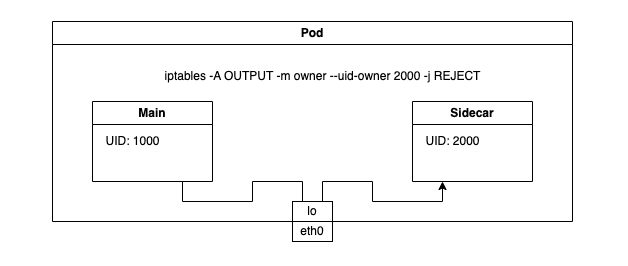
\includegraphics[width=\linewidth]{figures/iptables.png}
  \end{minipage}
  \hspace{\columnspace}
  % Right column
  \begin{minipage}[t]{\doublecolumnwidth}
    \vspace{\sectionspace}
    \section*{\sectiontitle{Solution 2}}

    Another approach is to split the network namespace by deploying containers in their own Pods. With \emphasis{macvlan} CNI and \emphasis{Multus}, a CNI plugin that allows creation of multiple network interfaces per Pod, a new bridge network can be created between the Pods. This network has own IP address space, and is independent from Network Policies applied on the default cluster network. For forwarding all \emphasis{localhost} traffic to the new network, a DNAT routing rule can be attached to the loopback devices. The functionality of Network Policies can be implemented on the bridge network with \emphasis{MultiNetworkPolicy}, a custom resource definition provided by the same team behind the Multus CNI.

    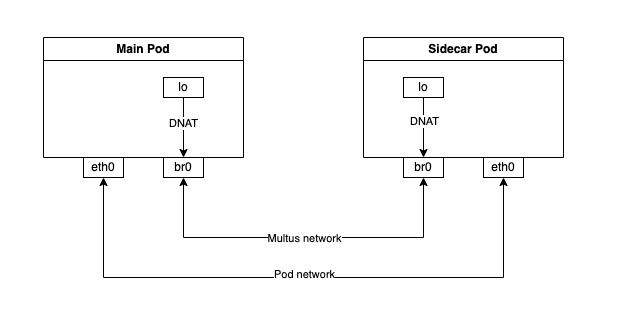
\includegraphics[width=\linewidth]{figures/multus.png}
  \end{minipage}
\end{minipage}

\makefooter
  {
    aarni.halinen@aalto.fi,
    jose.martinnavarro@aalto.fi,
    jacopo.bufalino@aalto.fi
  }
\end{document}
